\fancyhead[LE,RO]{Determination of pK with conductometry -- ,,PKVEZ''}
\fancyhead[LO,RE]{\thesection}
\fancyfoot[LE,RO]{\thepage}
\fancyfoot[RE,LO]{\emph{Physical chemistry lab. practice for pharmacy students}}

%\setcounter{section}{1}
\section{Determination of dissociation constants of weak acids with conductometry}
\subsection{Introduction}
According to Ohm's law, the current passing through between two points and the potential difference between those two points are in linear relationship:

\begin{equation}
\label{eq:ohm}
	U
	=
	I
	\cdot
	R
\end{equation}

where $R$ is the factor of proportionality, called \textbf{electrical resistance}. Its dimension is ohm ($\ohm$).

Specific resistance is the longitudinal resistance of a conductor which is 1 m long and has a cross section of 1 m$^2$ (1 mm$^2$ in practice). 

In electrochemistry it is often more simple to use the reciprocal of these quantities. The reciprocal of resistance is conductivity, its dimension is Siemens, S = 1/$\ohm$. The reciprocal of specific resistance is specific conductivity. The specific conductivity of an electrolyte is the conductivity we measure if the two electrodes have a surface area of 1 cm$^2$, they are 1 cm apart, they are made of an inert metal (gold, platinum), and they are submersed in the electrolyte. Its dimension is S $\cdot$ cm$^{-1}$. It depends on concentration, temperature, and it's a unique property of every material.

Molar specific conductivity ($\Lambda _m$) is the ratio of the specific conductivity and the concentration:

\begin{equation}
\label{eq:lambdam}
        \Lambda_m
        =
        \frac
		{\kappa 1000 }
		{c}
	=
	\kappa V
\end{equation}

where $c$ is concentration (mol$\cdot$dm$^{-3}$), and $V$ is dilution.

Kohlrausch found that the limiting molar conductivity (molar conductivity of an infinitely dilute solution) of anions and cations are additive: the conductivity of a solution of a strong electrolyte is equal to the sum of conductivity contributions from the cation and anion:

\begin{equation}
\label{eq:kohlrausch2}
	\Lambda _m^0
	=
	\lambda _a^0 \nu _a z_a + \lambda _k^0 \nu _k z_k
%	/1000
\end{equation}

where $z_a, z_k$ are the valence of the ions, $\nu _a, \nu _k$ are stochiometric factors, $\lambda _a^0$ and $\lambda _k^0$ are the limiting molar conductivities for the anions and the cations.

The conductivity of weak electrolytes can be described as follows:

\begin{equation}
\label{eq:lambdam}
        \lambda_c
        =
        \alpha
	\lambda_0
\end{equation}

where $\alpha$ is the degree of dissociation, $\lambda _0$ is the limiting molar conductivity.
The dissociation constant $K_d$ of a weak acid can be calculated from its concentration and its degree of dissociation:

\begin{equation}
\label{eq:kd}
        K_d
        =
        \frac{\alpha^2 c}{1-\alpha}
\end{equation}

It is worth noting however, that $K_d$ -- based on the Debye-Hückel theory -- depends on the permittivity of the media and temperature.

If we express $\alpha$ from \ref{eq:lambdam}, we get \emph{Ostwald's law of dilution}:

\begin{equation}
\label{eq:ostwald}
        K_d
        =
        \frac{\lambda_c^2 c}{\lambda_0^2 - \lambda_0\lambda_c}
\end{equation}

That means we can determine $K_d$ from conductometric measurements. $\lambda_c$ can be measured directly, while $\lambda_0$ can be obtained with the following method. By rearranging eq. \ref{eq:ostwald} we get

\begin{equation}
\label{eq:ostwald2}
        \frac{1}{\lambda_c}
        =
	\lambda_c
	c
	\frac{1}{K_d \lambda_0^2}
	+\frac{1}{\lambda_0}
\end{equation}

If we plot $1/\lambda_c$ as a function of $\lambda_c c$ (which is nothing but $\kappa$), we get a straight line whose y interception is $1/\lambda_0$. And knowing $\lambda_c$ and $\lambda_0$ we can calculate $K_d$.

Additionally, we have to consider these:

\begin{enumerate}[(a)]
\item The solvent also contributes to the conductivity of the solution. Therefore we substract the conductivity of the pure solvent ($G_{\text{solvent}}$) from each measurement carried out in the solutions of that solvent.

\item In practice, we don't use the conductivity cell from the definition of specific conductivity. Instead, the more practical ,,bell electrodes'' are used. To obtain specific conductivity from the conductivity values measured with these cells, we multiply every value with the cell constant $C$ (dimension:  m$^{-1}$ or cm$^{-1}$).

The cell constant shows the relationship between solution with a known specific conductivity ($\kappa_{ref}$) and the conductivity measured with cell used in practice ($G_{\text{measured}}$):

\begin{equation}
\label{eq:c}
	C
	=
	\kappa_{\text{ref}}/G_{\text{measured}}
\end{equation}

\end{enumerate}

Based on this, we can calculate the contribution of solute to the conductivity of the solution: $\kappa_{\text{korr}} = (G_{\text{solution}} - G_{\text{solvent}})C$, where $\kappa_{\text{korr}}$ is the specific conductivity of the solution taking into account that of the solvent and the cell constant.

Therefore, specific molar conductivity of a weak acid is:

\begin{equation}
\label{eq:c}
        \lambda
        =
        \kappa_{korr}
	V
\end{equation}


\begin{figure}[h!]
\centering
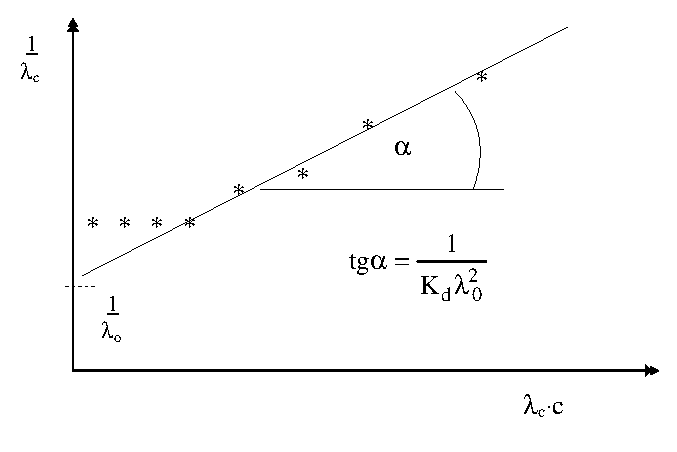
\includegraphics{lambda0.eps}
\caption{Obtaining the limiting molar conductivity ($\lambda_0$).}
\label{fig:}
\end{figure}

\subsection{Practice procedures}

Rinse the electrode of the conductometer several times (4 - 5) with deionized water, the with ultrapure water ($\kappa$ < 1 $\upmu$S/cm). Ask the technician for ultrapure deionized water.

Prepare 20 v/v\% solution from an alcohol selected by the instructor. Then prepare two weak acid solutions (the weak acid is also selected by the instructor), from the stock solution (1 mol$\cdot$dm$^{-3}$) by pipetting 2.00 cm$^3$ into two 100 cm$^3$ measuring flasks, and then filling one with the 20 v/v\% alcohol solution, the other with ultrapure deionized water up to 100 cm$^3$.

Carry out the conductivity measurements in a measuring cilinder. Pour the water based solution into the cilinder and measure its conductivity. Then, pipette 25 cm$^3$ from the cilinder into a clean 50 cm$^3$ measuring flask, fill it up with ultrapure deionized water (2$\times$ dilution), and measure the conductivity of the new solution after carefully rinsing it with ultrapure deionized water. Repeat the dilution and measurement 3 times. Then do the same with the alcohol based solution, but using the 20 v/v\% alcohol solution for the dilutions and rinsing.

Note and record the temperature measured by the built-in thermometer of the electrode for each measurement.

Finally, measure the conductivity of the solvents as well (for the correction).
Then, to obtain the cell constant, measure the conductivity of 0.01 M KCl solution, and write down the temperature as well. Based on table 

Figure \ref{fig:vez} shows the schematics of a conductometric cell. A well-defined, inert electrode pair is submersed into an electrolyte, and the voltage drop between them is measured. Alternating current is used to avoid polarization and electrolysis.

\begin{figure}
\centering
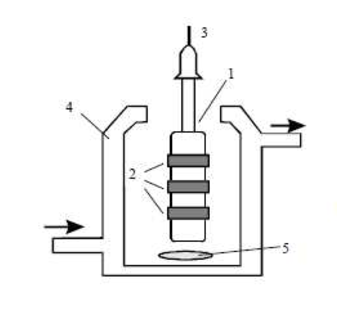
\includegraphics{cond.eps}
\caption{Schematics of a conductometric cell. 1 - ,,bell electrode'', 2 - platinized platinum rings, 3 - electrical connection, 4 - double walled vessel, 5 - magnetic stirrer.}
\label{fig:vez}
\end{figure}

\subsection{Evaluation}

\begin{enumerate}
\item Calculate the cell constant.
Present the recorded data in such a table:

\begin{table}[!h]
\centering
\begin{tabular}{|c|c|c|c|c|c|c|c|}
\hline
c (mol $\cdot$ dm$^{-3}$) & G$_{\text{measured}}$ & $\kappa_{\text{korr}}$ (S $\cdot$ cm$^{-1}$) & $\lambda_c$ & $1/\lambda_c$ & $\lambda_c c$ & $\alpha$ & $K_d$ \\
\hline
... & ... & ... & ... & ... & ... & ... & ... \\
\end{tabular}
\label{table:vez}
\end{table}

\item Determine $\lambda_0$ graphically. Knowing $\lambda_c$ and $\lambda_0$, calculate $\alpha$ and $K_d$ for each concentration.

\end{enumerate}


